Trois condensateurs, $C_1 = \qty{\v{C1}}{\micro\farad}$, $C_2 = \qty{\v{C2}}{\micro\farad}$ et $C_3 = \qty{\v{C3}}{\micro\farad}$, sont branchés en série aux bornes d'une pile de \qty{\v{V}}{V}.

\begin{center}
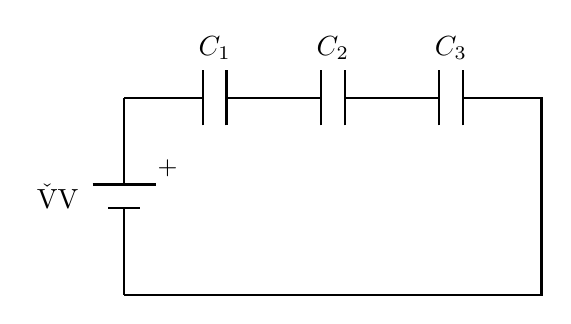
\begin{tikzpicture}[thick, res/.style={decorate,decoration={zigzag,segment length=5pt,amplitude=4pt,pre length=0.4cm,post length=0.4cm}}]
    \draw (0,0) -- (0,1.10);
    \draw (-0.2,1.10) -- (0.2,1.10);
    \draw (-0.4,1.40) -- (0.4,1.40);
    \draw (0,1.40) -- (0,2.5);
    \node[left] at (-0.45,1.25) {\qty{\v{V}}{V}};
    \node at (0.55,1.60) {\small$+$};
    \draw (0,2.5) -- (1,2.5);
    \draw (1,2.15) -- (1,2.85); \draw (1.3,2.15) -- (1.3,2.85);
    \draw (1.3,2.5) -- (2.5,2.5);
    \draw (2.5,2.15) -- (2.5,2.85); \draw (2.8,2.15) -- (2.8,2.85);
    \draw (2.8,2.5) -- (4,2.5);
    \draw (4,2.15) -- (4,2.85); \draw (4.3,2.15) -- (4.3,2.85);
    \draw (4.3,2.5) -- (5.3,2.5) -- (5.3,0) -- (0,0);
    \node[above] at (1.15,2.85) {$C_1$};
    \node[above] at (2.65,2.85) {$C_2$};
    \node[above] at (4.15,2.85) {$C_3$};
\end{tikzpicture}
\end{center}

\begin{enumerate}[label=\alph*)]
    \item Déterminez la capacité équivalente du montage.
    \item Déterminez la charge sur chaque condensateur.
    \item Déterminez la différence de potentiel aux bornes de chaque condensateur et vérifiez que leur somme donne la tension de la pile.
\end{enumerate}
